\subsection{Experiment}
In the second part of the experiment we have the goal to measure the wavelengths of the mercury spectrum with a grating spectrometer.
Figure \ref{fig::scope} shows the structure of the used spectrometer. 
\begin{figure} [ht]
	\centering
	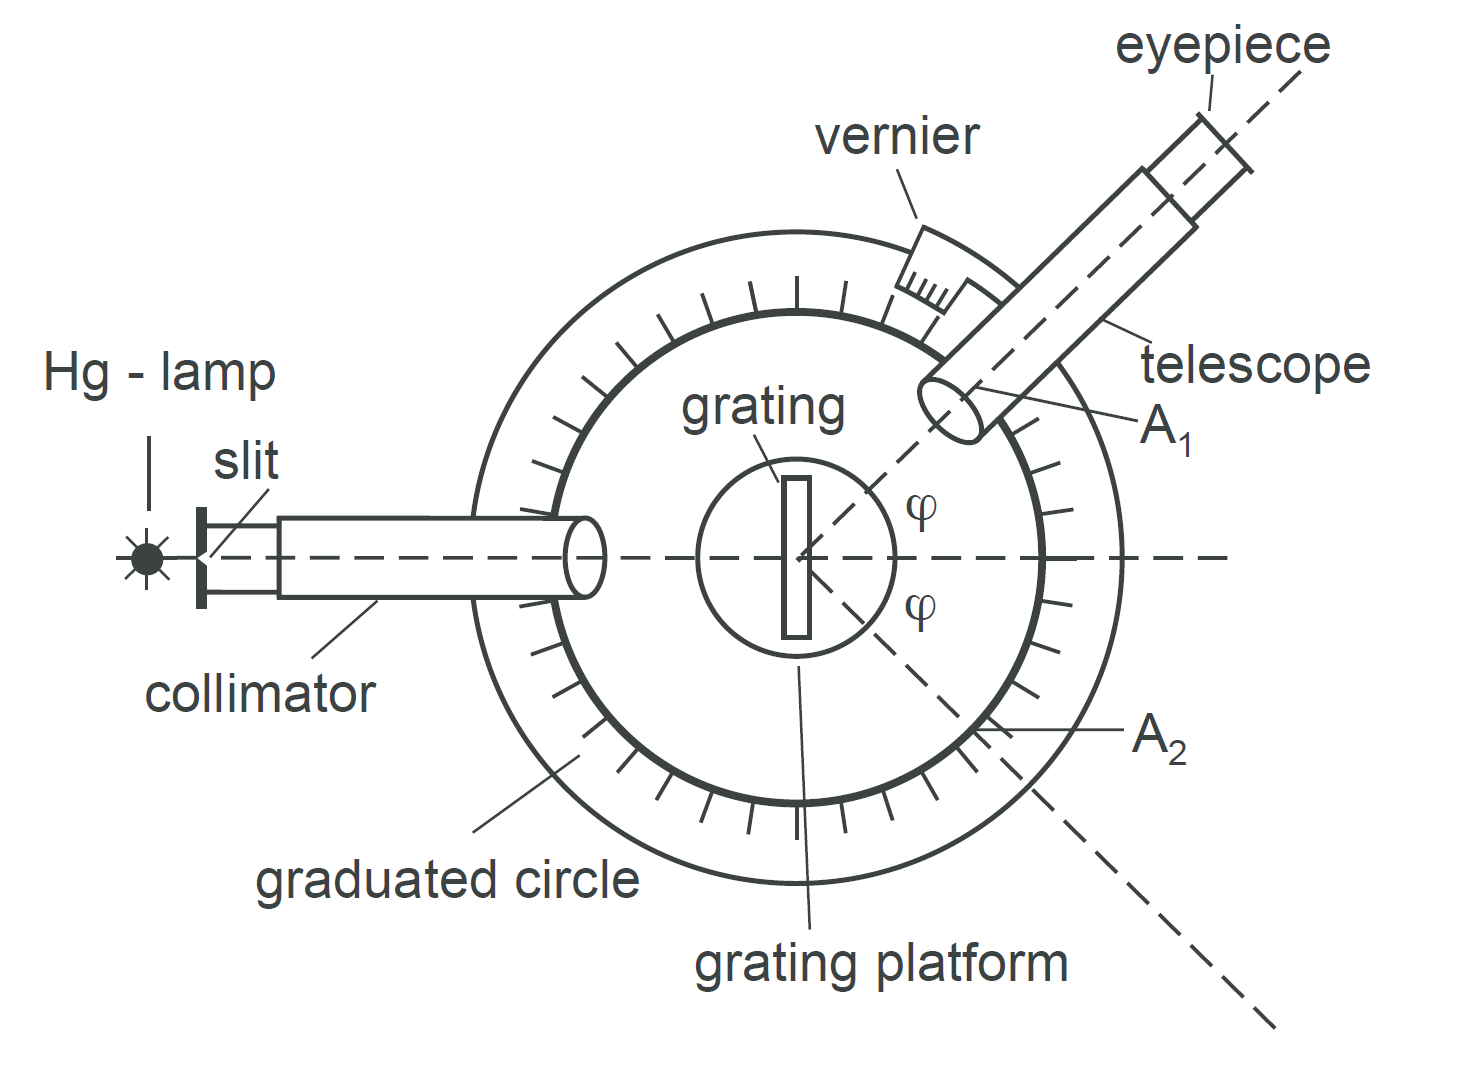
\includegraphics[height=200pt]{img/scope.png}
	\caption{Spectrometer used according to the manual \cite{manual}.}
	\label{fig::scope}
\end{figure}

The mercury (Hg)-lamp produces a bright light which goes trough the slit and collimator and illuminates the grating (displayed in figure \ref{fig::scope}).
It is important for this measurement technique, that the light impinges perpendicular on the grating.
Thus we have to adjust the setup accordingly to the procedure given by the manual\cite{manual}.
The setting includes the following five steps described further in the manual \cite{manual}:
\begin{itemize}
	\item Focusing the telescope to infinity
	\item Vertical alignment of the telescope axis to the spectrometer axis
	\item Adjusting the collimator
	\item Vertical alignment of the grating to the collimator axis
	\item Adjusting the grating
\end{itemize}
After doing this steps the telescope should be ready to measure.

To see the spectrum lines trough the scope, we rotate the scope away from the zero point which looks directly in the light source.
Next we have to align the visible coloured lines seen trough the scope, with the cross hair of the scope.
When they are aligned, we read the angle $A_1$ from the vernier on top of the spectrometer.
The telescope gets rotated in the other direction until the same spectral line is seen and again the angle $A_2$ is taken.
We call this measured angle $A_1$ and $A_2$ for each side and colour.


The measured angles are then used to determine the wavelength of the coloured line observed.
 